\documentclass[10pt]{scrartcl}
\usepackage{amsmath,amssymb,amsthm}
\usepackage{graphicx}
\usepackage[margin=1in,letterpaper]{geometry}
\usepackage{subfigure}

\theoremstyle{remark}
\newtheorem{remark}{Remark}

\setlength{\parskip}{.1in}
\setlength{\parindent}{0in}
\providecommand{\R}{\ensuremath \mathbb{R}}
\providecommand{\ip}[1]{\ensuremath \langle #1\rangle}

\begin{document}
\title{Towards computing the BRS of nonlinear systems driven by uncertain dynamics}
\subtitle{Convex computation of the BRS with constant uncertainties}
\author{Shankar Mohan, Ram Vasudevan}
\maketitle
The question that this note attempts to address is the following -- how does one compute the time limited BRS under constant parametric uncertainty? The approach taken is a direct extension of the formulation in [Henrion], save for the difference in the way the dynamics of the system is described.

\section{Basic problem formulation}

We consider a polynomial dynamical system whose state evolution is described by the following
\begin{align}
	\dot x=f(x\mid\theta)
\end{align}
wherein $x\in \R^{n_x}$ are the states of the model, $\theta\in \R^{n_\theta}$ are the parameters that are not known a priori but whose probability distribution is given by $\mu_{\theta}$; it is assumed that the distribution of $\theta$ is not state dependent. As stated, $f$ and $g$ are polynomial functions and the states are assumed to be restricted to evolve in semi-algebraic sets $\mathcal X$.
\par
The choice of a drift system is deliberate---to simplify presentation---and the presented method can be extended to a control affine system with ease.
\par 
To assist in our problem formulation, we define the following 
\begin{align}
\begin{bmatrix}\dot x\\\dot\theta\end{bmatrix}=\tilde f(x,\theta):=&\,\begin{bmatrix}f(x\mid\theta)\\0
\end{bmatrix}\\
	\mu(A\times B\times C\mid x_0,\theta_0):=&\,\int_{0}^T I_{A\times B\times C}(t,x(t\mid x_0,\theta_0),\theta_0) \,dt
\end{align}
where $A\subset \mathcal T:=[0,T]$, $B\subset \mathcal X$ and $C\subset \Theta$. The $\mu(\cdot\mid x_0)$ is a measure of the time spent by the state trajectory in the set $B\times C$ if the initial condition of the system was $x_0$ and the value of the uncertain parameter was $\theta_0$. Since the initial distribution of $x$ is independent of that of $\theta$,
\begin{align}
	\mu(A\times B\times C):=&\,\int_{\mathcal X} \mu(A\times B\times C\mid x_0) \,d\mu_0(x_0,\theta_0)\\
	\mu_T(A\times B):=&\,\int_{\mathcal X\times \Theta}I_{A\times B}(x(T\mid x_0,\theta_0),\theta(T\mid \theta_0))\,d\mu_0(x_0,\theta_0)
\end{align}
$\mu(\cdot)$ is the \emph{average occupation measure} and corresponds to the total time that is spent by all system trajectories that arise from the support of $\mu_0$, the measure on the set of admissible initial conditions.
\par
Consider a test function $v\in C^1(\mathcal T\times \mathcal X\times \Theta); \mathcal T\times \mathcal X\times \Theta\mapsto \R$ and its evolution along the flow of states. By the fundamental theorem of calculus, one has
\begin{align}
	v(T,x(T\mid x_0,\theta_0),\theta(T))=v(0,x_0,\theta_0)+\int_{0}^T \mathcal L_{\tilde f}v(t,x(t\mid x_0,\theta_0),\theta(t\mid \theta_0))\,dt
\end{align} 
where $\mathcal L_{\tilde f}v:=\frac{\partial v}{\partial t}+\nabla_x v \cdot \tilde f$.
\par
 By definition, the following equalities hold
\begin{align}
	v(T,x(T\mid x_0,\theta_0),\theta(T))=&\,v(0,x_0,\theta_0)+\int_{0}^T \mathcal L_{\tilde f}v(t,x(t\mid x_0,\theta),\theta(t\mid\theta_0))\,dt\\
	=&\,v(0,x_0)+\int_{\mathcal T\times \mathcal X\times \Theta}\mathcal L_{\tilde f}v(t,x,\theta)\,d\mu(t,x,\theta\mid x_0,\theta_0)
\end{align}
By considering the bundle of trajectories emanating from the set of admissible initial conditions (integrating wrt. $\mu_0$),
\begin{align}
	\int_{\mathcal X_T\times \Theta} v(t,x,\theta) \,d\mu_T=\int_{\mathcal X\times \Theta}v(0,x_0,\theta_0)\,d\mu_0(x)+\int_{\mathcal T\times \mathcal X\times \Theta} \mathcal L_{\tilde f}v(t,x,\theta)\,d\,\mu(t,x,\theta).
\end{align}
Now, we formulate the primal problem as described in [Henrion]
\begin{flalign}
	\sup \ip{\mu_0,1}\\
	&&\mu_T=&\,\delta_0\otimes\mu_0\otimes \mu_\theta+\mathcal L_{\tilde f}'\mu&\\
	&& \mu_0+\hat\mu_0=&\,\lambda
\end{flalign}
The dual to the above primal is 
\begin{flalign}
\inf \ip{\lambda,w}\\
&& w\ge &\,0&\\
&& v(T,\cdot,\cdot)\ge&\, 0 & \forall (x,\theta)\in \mathcal X_T\times \Theta\\
&& - \mathcal L_{\tilde f}v\ge&\,0 & \forall (x,\theta)\in \mathcal X\times \Theta\\
&& w-1-\int_\Theta v(0,\cdot,\theta)\,d\mu_\theta(\theta)\ge &\,0 & \forall x\in \mathcal X
\end{flalign}
To find the outer approximation of the BRS:
\begin{align}
0\le v(T,x(T),\theta(T))=&\,v(0,x_0,\theta_0)+\int_{0}^T\mathcal L_{\tilde f}v(t,x,\theta))\,dt\\
\le &\,v(0,x_0,\theta_0)\\
0\le \int_{\Theta}v(T,x(T),\theta(T))\,d\mu_\theta\le &\,\int_{\Theta}v(0,x_0,\theta_0)\,d\mu_\theta\\
\le w(x_0)-1
\end{align}
\newpage

\subsection{Examples}
In the following examples, it is assumed that $\theta\in [0,1]$.
\subsubsection{1D system with additive uncertainty}
\begin{align}
	\dot x =&\, ax+m\theta+c\\
	x(t)=&\, \left(x_0+\frac{m\theta}{a}\right)e^{at}-m\theta
\end{align}
Let the terminal set be $[0.2,0.4]$ at the terminal time be $T=1$. Then
\begin{align}
\forall \theta\in \Theta,\, BRS_\theta=&\,\left[(0.2+\theta)e^{-a}-\frac{m\theta}{a},(0.4+\theta)e^{-a}-\frac{m\theta}{a}\right]
\end{align}
For the specific case of $a=m=1$ and $c=0$
\begin{align}
BRS_\theta=&\,[0.0736-0.632\theta,0.145-0.632\theta]
\end{align}

\begin{figure}[!ht]%
\centering
\subfigure[]{\frame{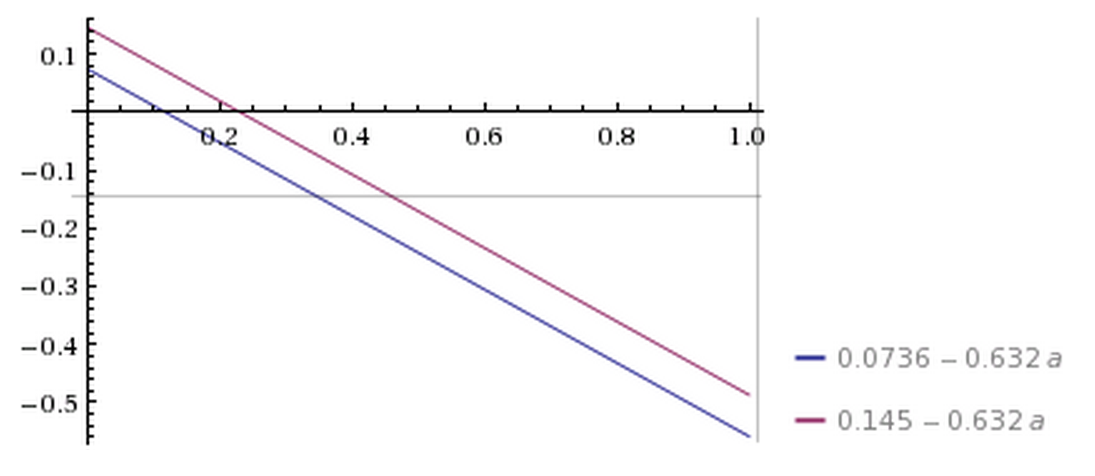
\includegraphics[width=.5\columnwidth]{figures/ex_1}}}
\subfigure[]{{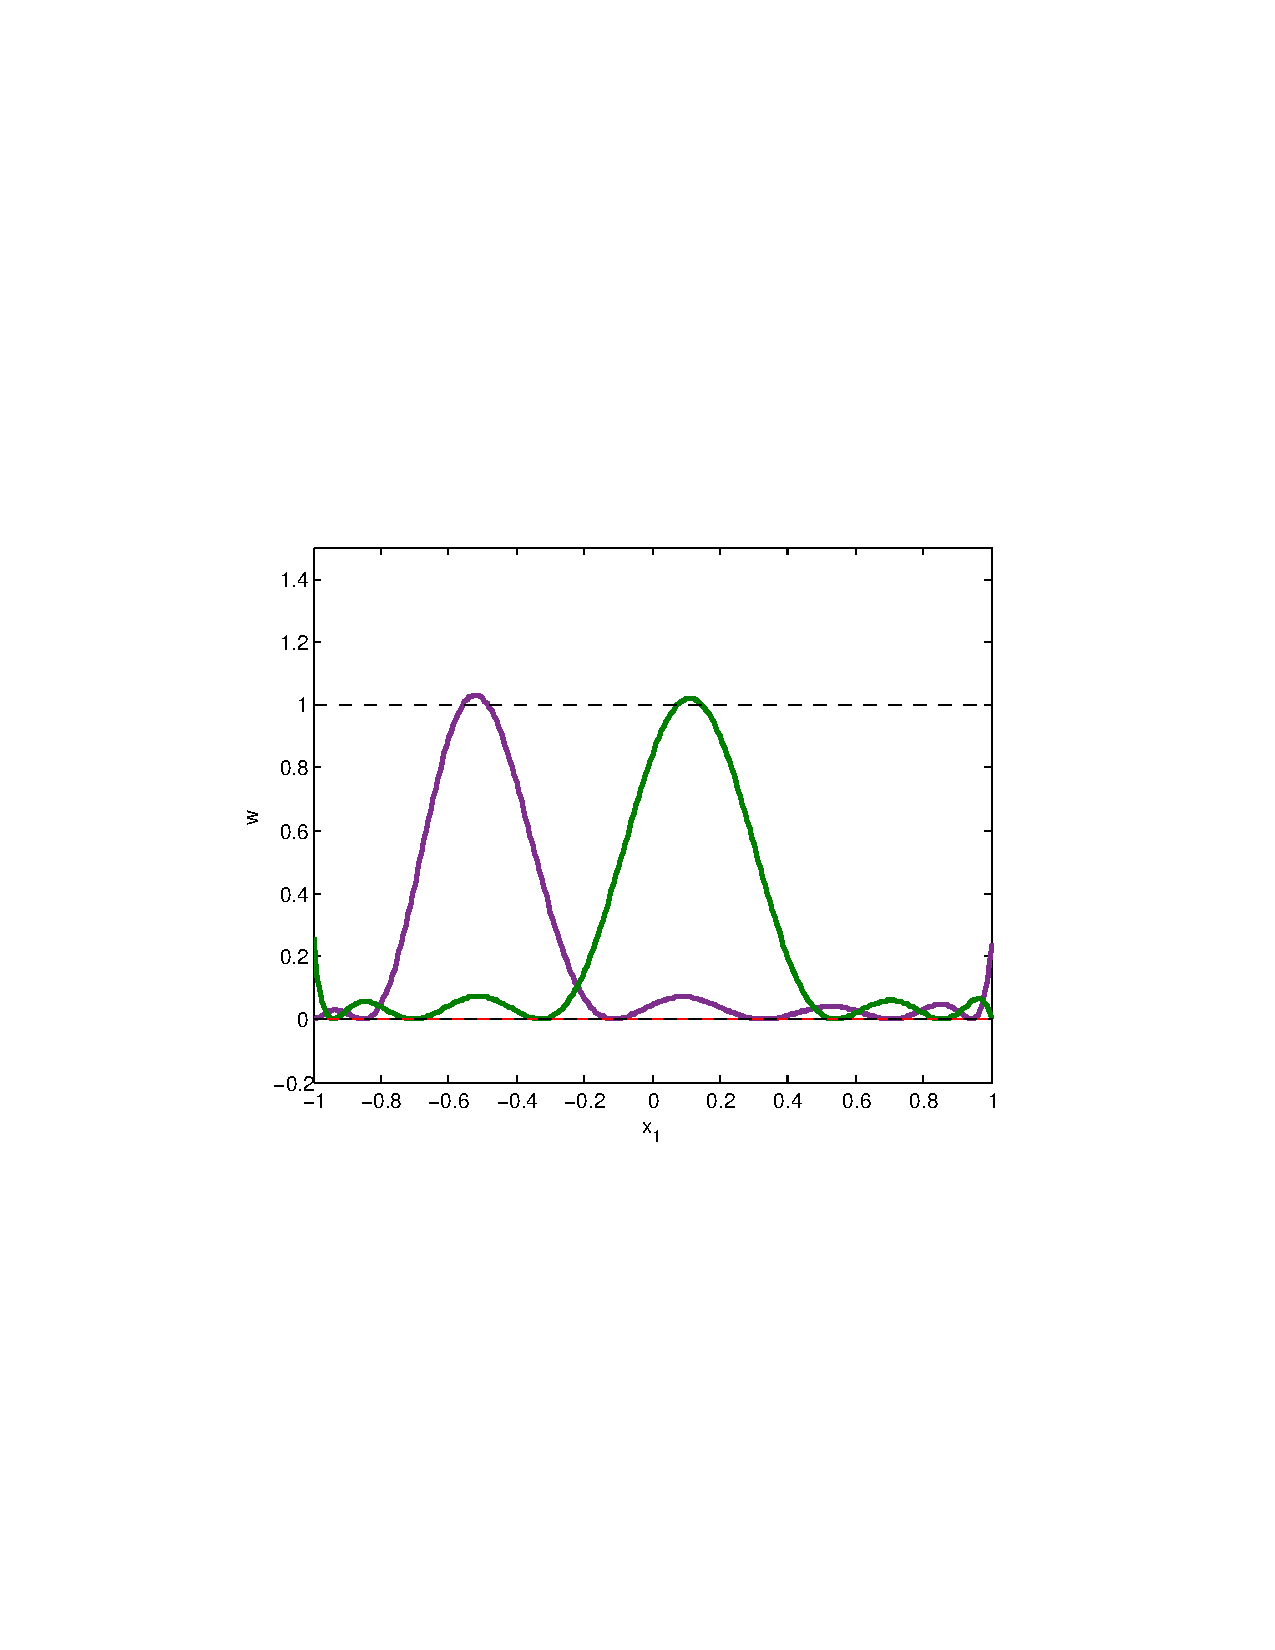
\includegraphics[width=.5\columnwidth,trim= 1.5in 3.3in 1.5in 3.5in]{figures/1D_1}}}
\caption{w function for $\theta=1$ (purple), $\theta=0$ (green) $\mu_\theta$ and (red)}%
\end{figure}

Now, if the BRS of the uncertain system is defined as the intersection of $BRS_\theta,\,\forall \theta\in \Theta$, then $BRS=\emptyset$.
\newpage
\clearpage
However, if the $m=0.1$ and $a=-1$
\begin{figure}[!ht]%
\centering
\subfigure[]{\frame{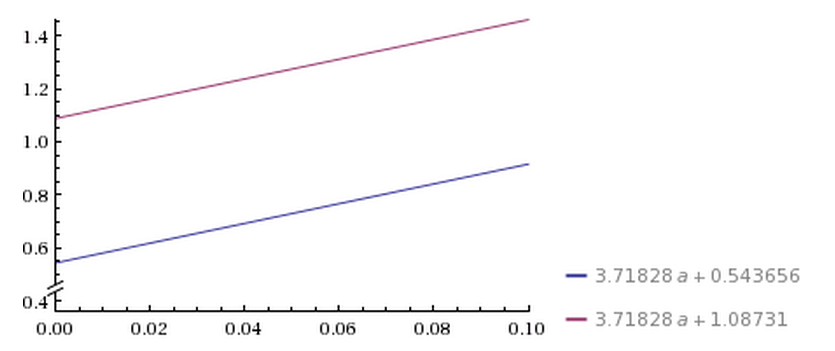
\includegraphics[width=.5\columnwidth]{figures/ex_1_1}}}
\subfigure[]{{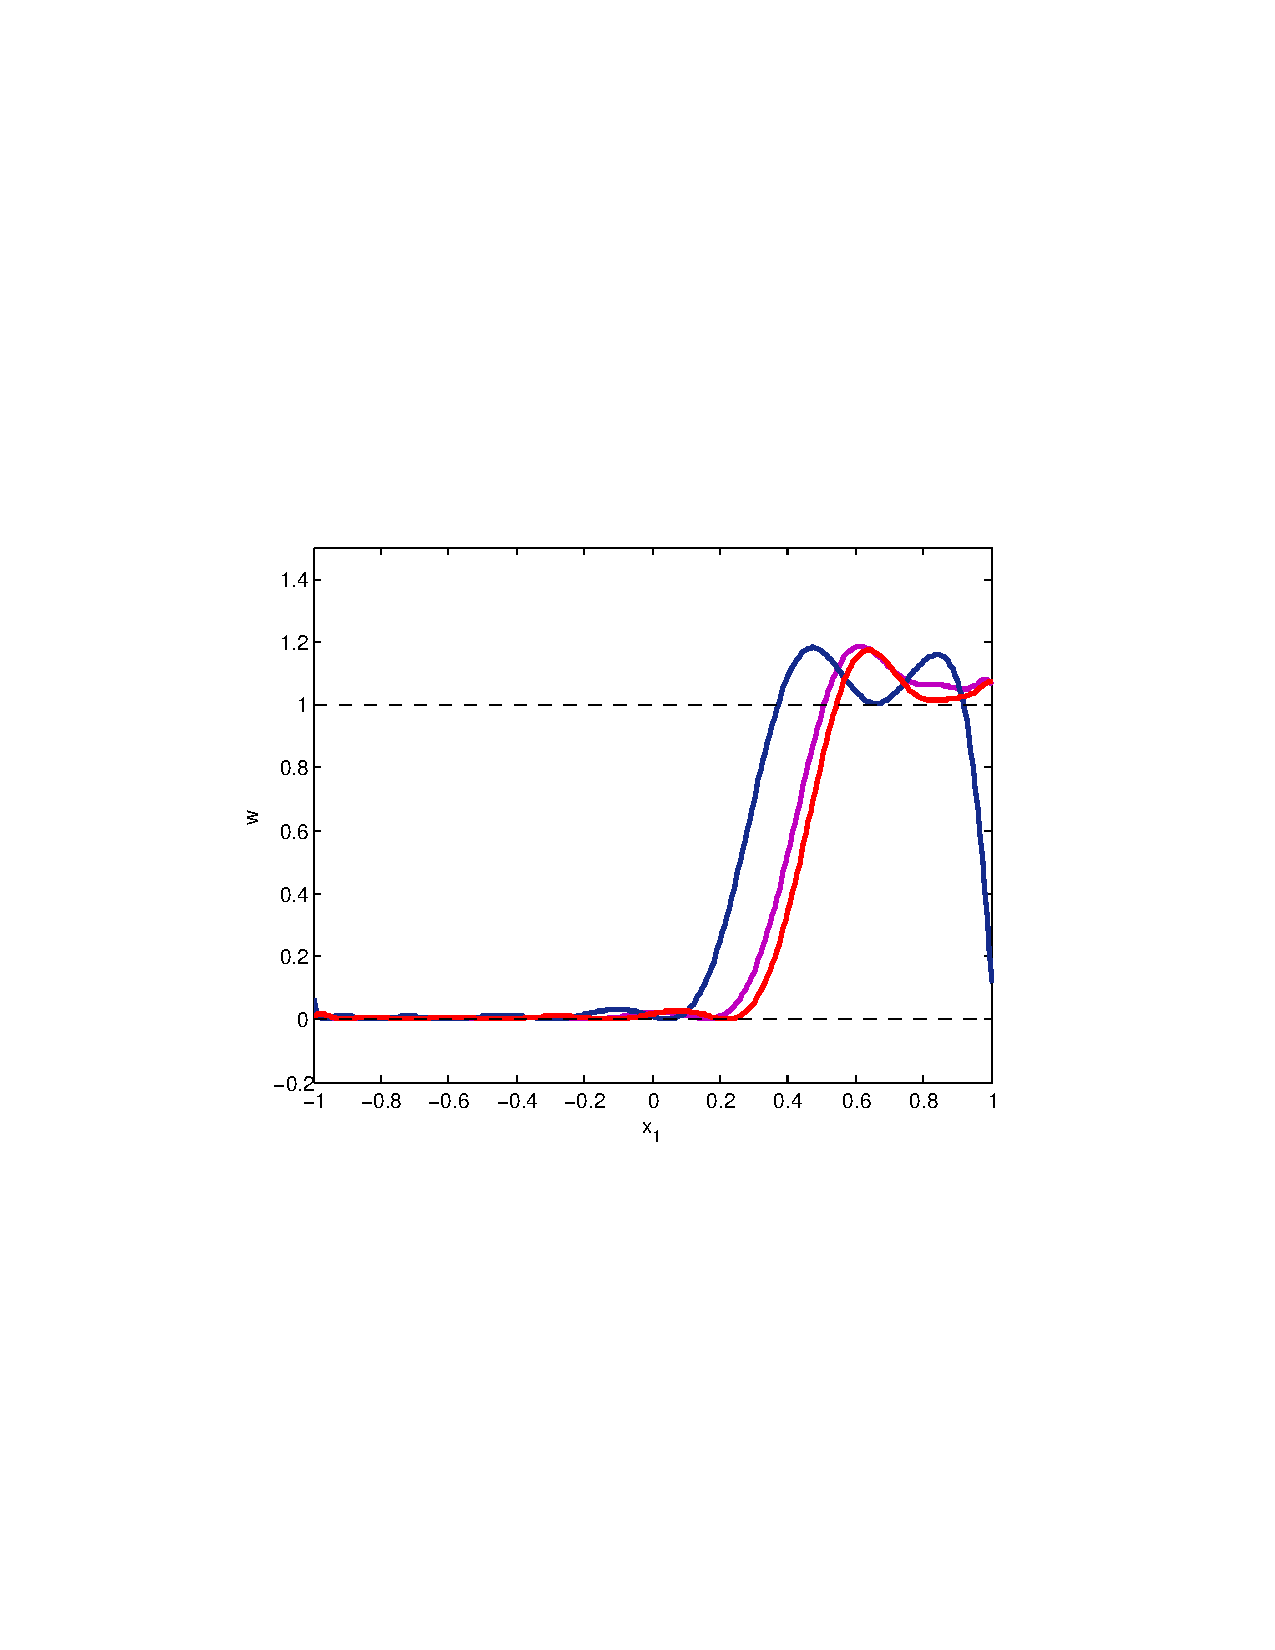
\includegraphics[width=.5\columnwidth,trim= 1.5in 3.3in 1.5in 3.5in]{figures/1D_2}}}
\caption{(a) BRS for each $\theta$ (read `a' as $\theta$) (b) (purple) $\mu_\theta$, (red) $\theta=0$ and (navy) $\theta=1$}%
\end{figure}
\newpage
\clearpage
However, if the $m=1/5$, $c=-0.1$ and $a=-0.7$
\begin{figure}[!ht]%
\centering
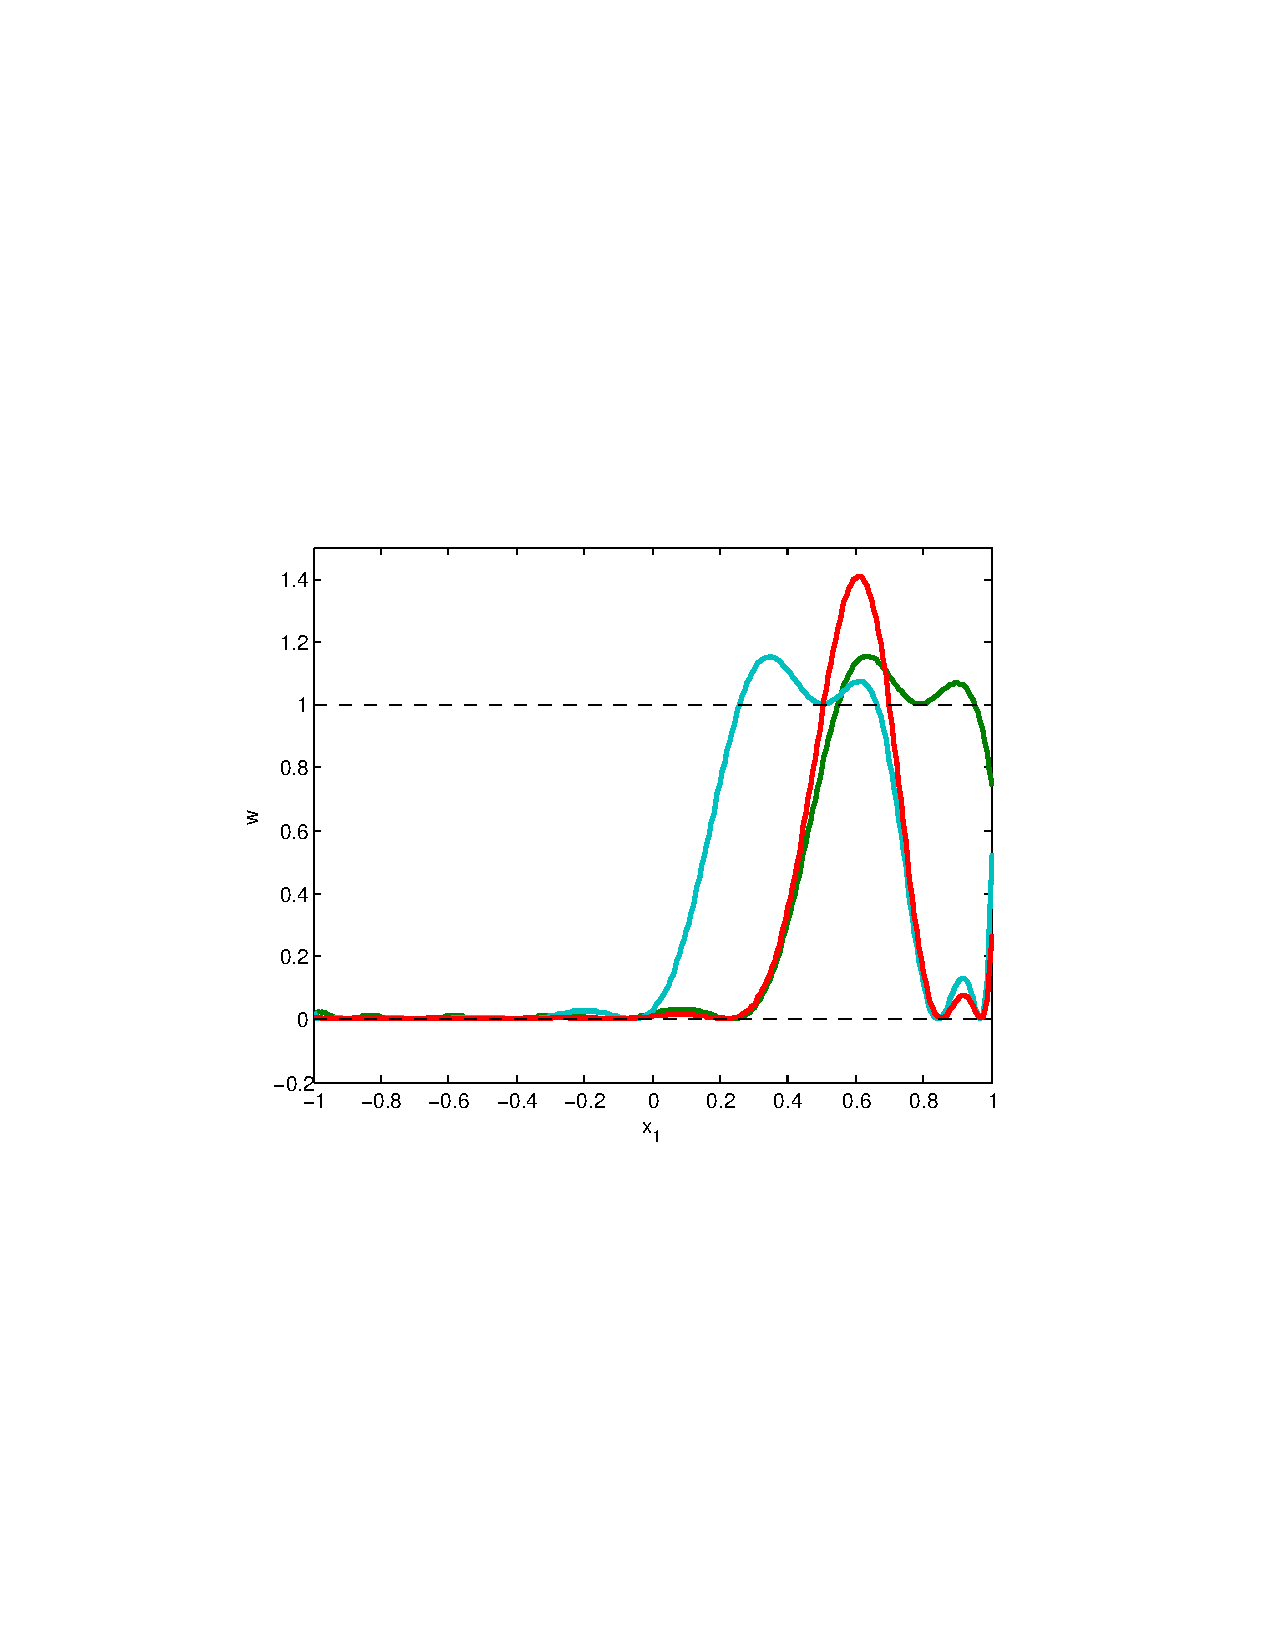
\includegraphics[width=.5\columnwidth,trim= 1.5in 3.3in 1.5in 3.5in]{figures/1D_3}
\caption{(green) $\theta=0$, (blue) $\theta=1$ and (red) $\mu_\theta$}%
\end{figure}

\par
\centerline{\rule{.5\columnwidth}{1pt}}
%\newpage
%\clearpage
\subsubsection{2D linear system with structural uncertainty}
\begin{align}
\begin{bmatrix}
\dot x_1\\\dot x_2
\end{bmatrix}=\begin{bmatrix} -1 & 1\\-.2 & -\theta+0.5
\end{bmatrix}\begin{bmatrix}
x_1\\x_2
\end{bmatrix}
\end{align}

\begin{figure}[!ht]
\centering
\subfigure[]{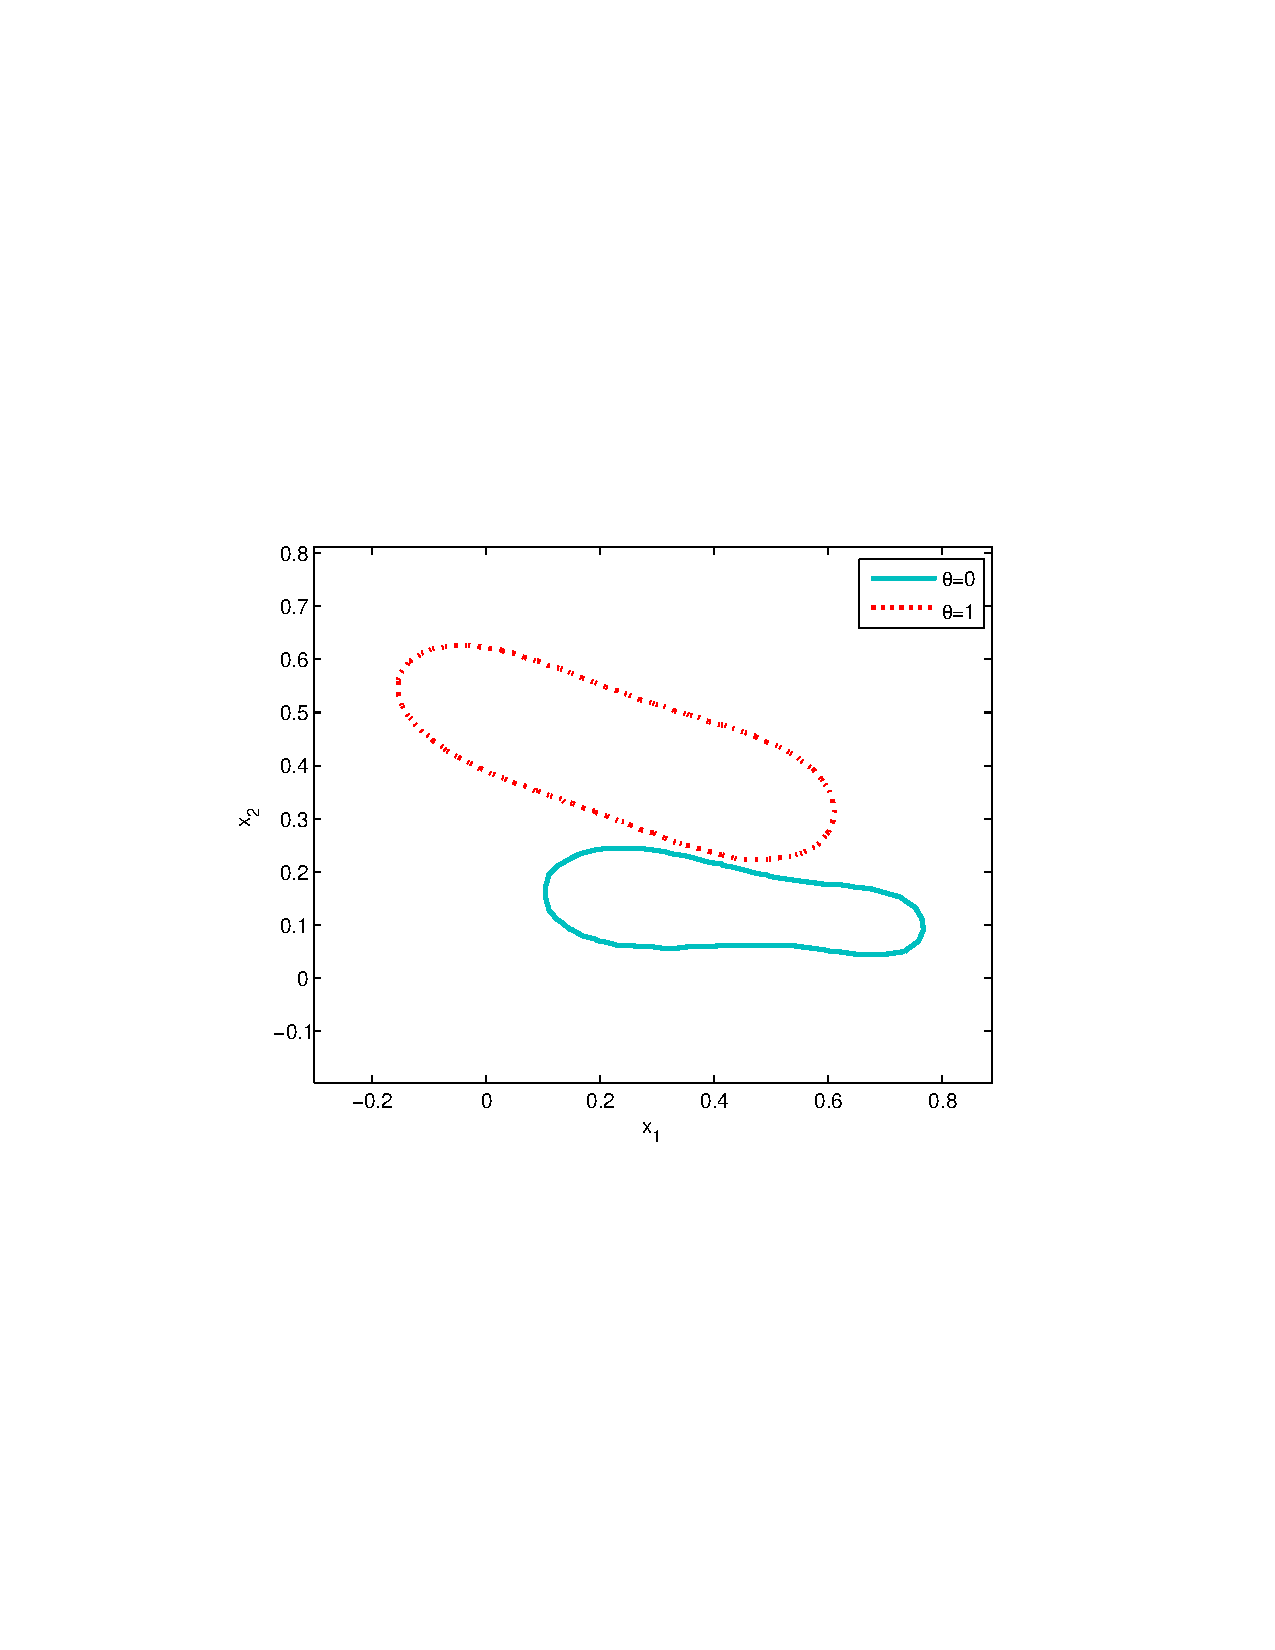
\includegraphics[trim=1.5in 3.3in 1.5in 3.5in, width=.48\columnwidth]{figures/2D_1}}
\subfigure[]{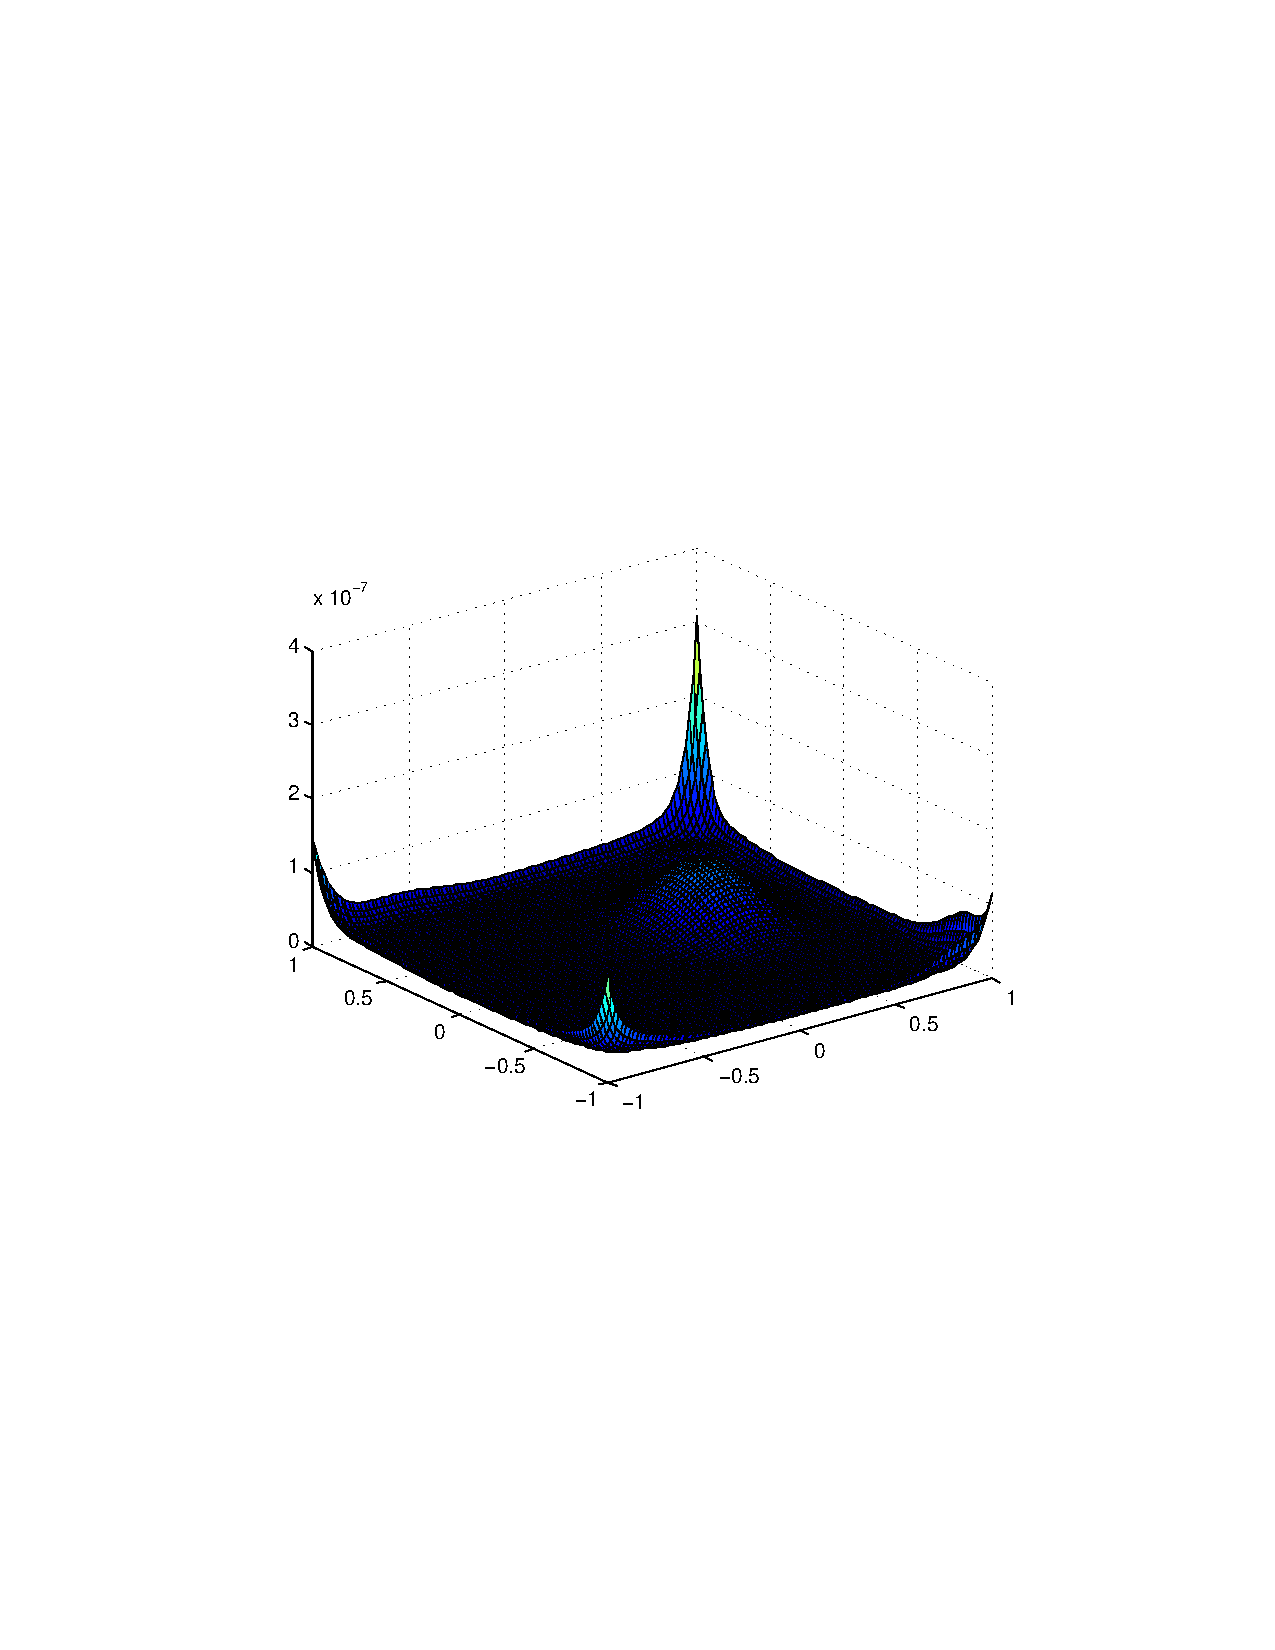
\includegraphics[trim=1.5in 3.3in 1.5in 3.5in, width=.48\columnwidth]{figures/2D_1_1}}
\caption{(a) BRS for different values of $\theta$ (b) w function}%
\end{figure}

\subsubsection{Non-linear 2D system}
\begin{align}
	 \begin{bmatrix}\dot x_1\\\dot x_2
	\end{bmatrix}
	=
	\begin{bmatrix}
	\theta^3x_1-(1-\theta)x_2^3+\frac{x_1^5}{120}-x_2^7\\
    0.1-(1-\theta)^2x_2+\theta x_1^2+\frac{x_1^6}{12}-x_2^6
	\end{bmatrix}
\end{align}
where $\theta\in [0.7,1]$.
\begin{figure}[!ht]
\centering
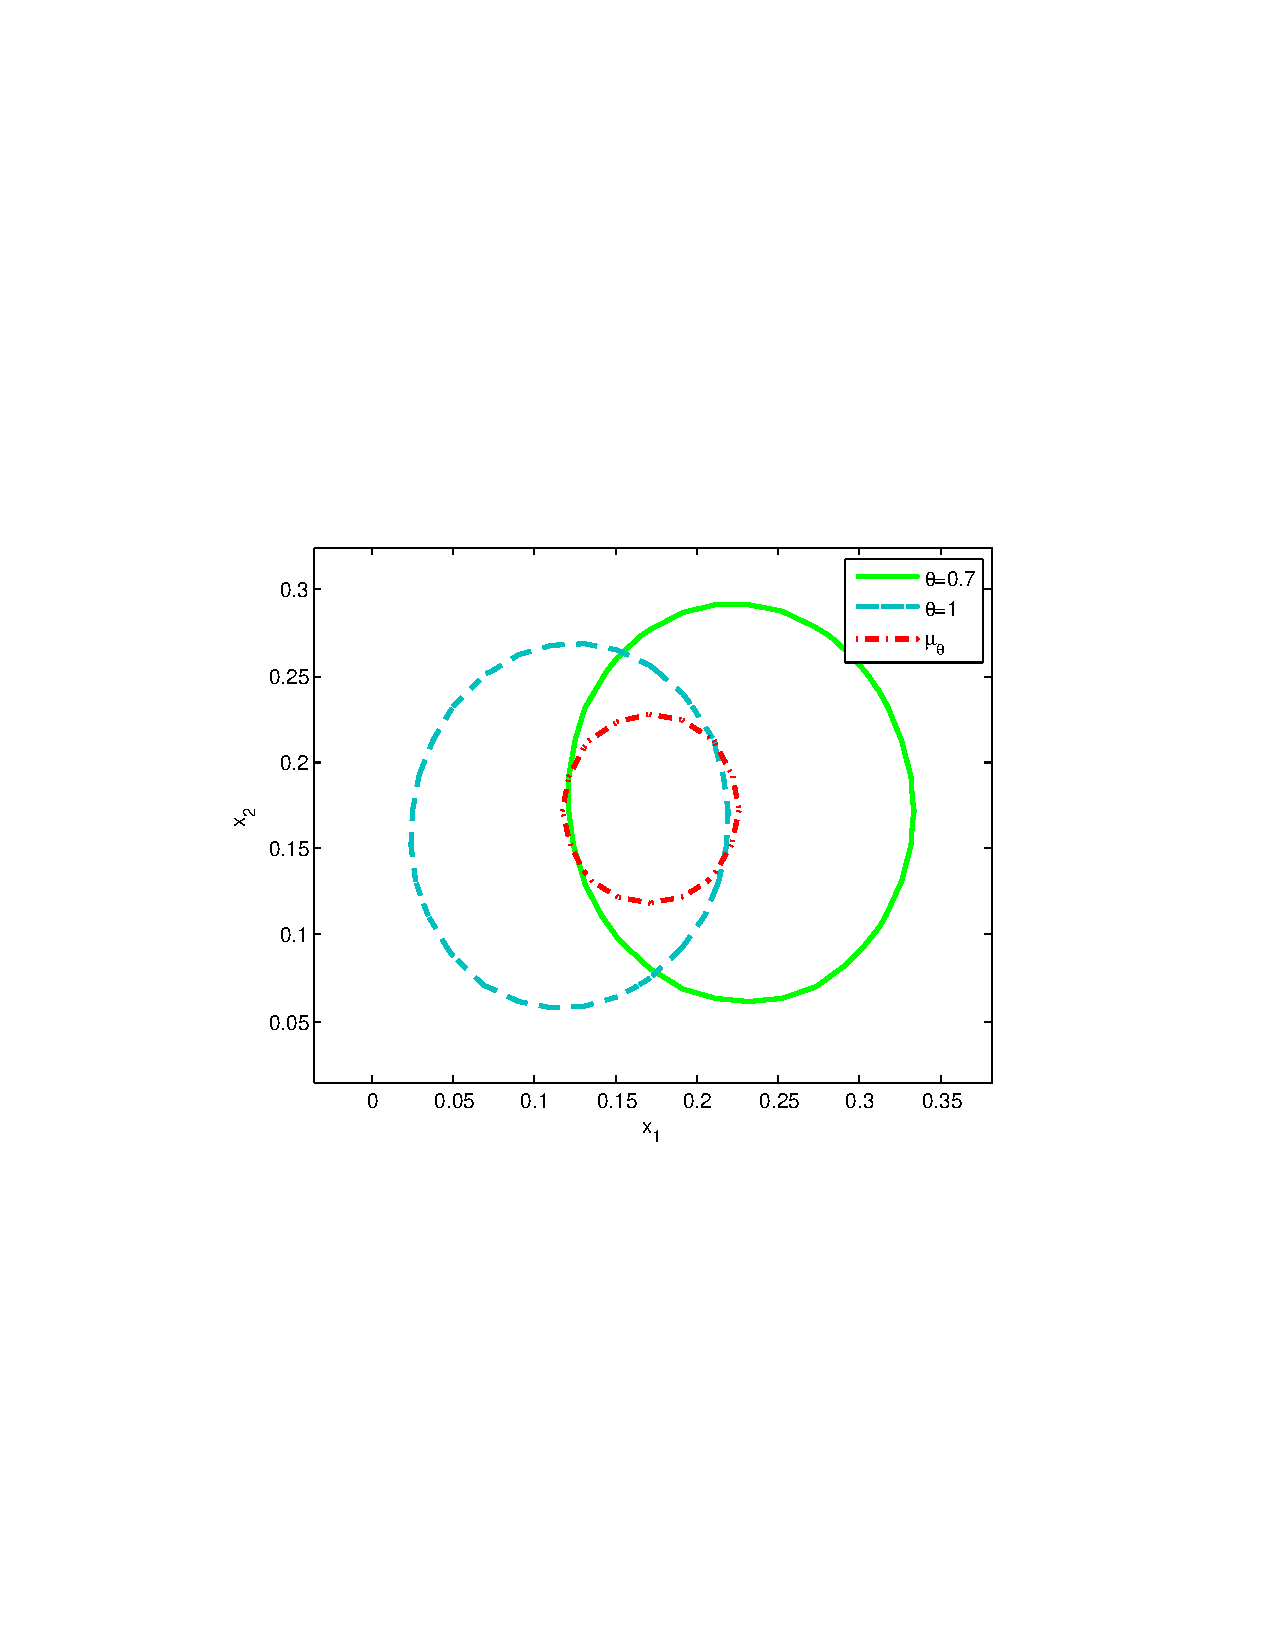
\includegraphics[trim=1.5in 3.3in 1.5in 3.5in, width=.5\columnwidth]{figures/2D_2}%
\caption{(degree 12) Outer approximation of BRS (red). The other contours are the BRS for different values of $\theta$}%
\end{figure}

\newpage
\section{$\alpha$ confidence level}
The last section addressed the case wherein the goal was to estimate the set of initial conditions (state) were independent of parameters (read uncertainties drawn from a distribution $\mu_\theta$) that reaches a certain terminal set $\mathcal X_T$. Clearly, for one initial condition and a given $\mu_\theta$, the distribution of terminal states is related to the advection of $\mu_\theta$ along the flow of the state trajectories. By extension, given a set of initial conditions, the set of terminal states is going to be distributed over a set, not necessarily uniformly.\par
In this section, we attempt to identify the set of initial conditions that can guarantee that the terminal state lies in $\mathcal X_T$ with some $\alpha $ confidence.
To that end, we redefine one of the measures of interest -- the terminal measure:
\begin{align}
\mu_T(A\times B)=\int_{\mathcal X\times \Theta} I_{A\times B}(x(T\mid x_0,\theta_0),\theta(T\mid \theta_0))\,d\,\mu_0\times \mu_\theta	
\end{align}
only this time, $\mu_T\in \mathcal M(\mathcal X\times \Theta)$ as opposed to the last section wherein $\mu_T\in \mathcal M(\mathcal X_T\times \Theta)$. With this redefinition, the primal problem is as stated in the following.
\begin{flalign}
	\sup \ip{\mu_0,1}\\
	&&\delta_T\otimes(\mu_{T_1}+\mu_{T_2})=&\,\delta_0\otimes\mu_0\otimes \mu_\theta+\mathcal L_{\tilde f}'\mu&\\
	&& \mu_0+\hat\mu_0=&\,\lambda\\
	&& \alpha\ip{\mu_{T_1}+\mu_{T_2},1}+r=&\,\ip{\mu_{T_1},1}
\end{flalign}
where $\mu_{T_1}\in \mathcal M(\mathcal X_T\times \Theta), \mu_{T_2}\in \mathcal M(\mathcal X\backslash \mathcal X_T\times \Theta),\mu_0,\hat \mu_0\in \mathcal M(\mathcal X)$ and $r\in \R_{\ge 0}$.\\ 
The dual to the above reads as follows
\begin{flalign}
\inf \ip{\lambda,w}\\
&& w\ge &\,0&\\
&& v(T,\cdot,\cdot)+q(\alpha-1)\ge&\, 0 & \forall (x,\theta)\in \mathcal X_T\times \Theta\\
&& v(T,\cdot,\cdot)+q\alpha\ge&\, 0 & \forall (x,\theta)\in \mathcal X\times \Theta\backslash\mathcal X_T\times \Theta\\
&& - \mathcal L_{\tilde f}v\ge&\,0 & \forall (x,\theta)\in \mathcal X\times \Theta\\
&& w-1-\int_\Theta v(0,\cdot,\theta)\,d\mu_\theta(\theta)\ge &\,0 & \forall x\in \mathcal X
\end{flalign}
where $v\in C^1(T\times \mathcal X\times \Theta)$, $w\in C(\mathcal X)$ and $q\in \R_{\ge 0}$.\par
Approximation of the set of initial conditions which reach $\mathcal X_T$, 
$$S_1=\{x\mid w(x)\ge 1+q(1-\alpha)\}$$
Approximation of the set of initial conditions which do not reach $\mathcal X_T$, 
$$S_2=\{x\mid w(x)\ge 1-q\alpha\}$$
Now, since $q\in \R_{\ge 0}$, it follows that $S_1\subset S_2$ and hence set of initial conditions of interest (BRS) to us is contained in $S_2$.

\newpage

\section{Further thoughts : Hybrid systems}
We now turn our attention the problem of estimating the BRS of a hybrid system with uncertainty; particularly, we consider the example if a walking biped moving along a terrain that has bounded variations in height. For simplicity, let the hybrid system under consideration consist of just one mode; the dynamics in that mode is give by (As ever, we restrict our attention to drift systems for brevity of presentation although the complications associated with having a control vector field need investigation and will be pursued later in this section.)
\begin{align}
\dot x=f(x).
\end{align}
When the states reaches the guard ($G$), they are reset using a reset map $G\rightarrow R(G)$. Within the confines of the problem description, the uncertainty in terrain height does not affect the dynamics of the system. Specifically, if the approach of augmenting the state-space with a parameter as pursued in Section 1 was adopted, then can be shown that $$\mu=\bar\mu\otimes \mu_\theta.$$
The only place where the uncertainty features is in the definition of the guard; i.e. $\forall \theta\in \Theta$, the guard is $G_\theta$ and let us define the measure on the $G_\theta$ by $\mu^G_\theta$ (Borel $\sigma$-algebra is assumed). Consequently, for each value of $\theta$, define the measure after reset $\mu^{G*}_{\theta}$ such as to satisfy the following relationship
\begin{align}
	\int_{R(G_\theta)} v(t,x)\,d\mu_{\theta}^{G*}(t,x(t\mid \theta))=\int_{G_\theta}v(t,R(x))\,\cdot J(x)\,d\mu_\theta^G(t,x(t\mid \theta))
\end{align}
where $J$ is the Jacobian determinant of $R$.
\par
Consider the primal
\begin{flalign}
	\sup \ip{\mu_0,1}\\
	&&\begin{split}
	\int_{\mathcal X_T}v(T,x)\,d \mu_{T}+&\,\int_{\mathcal T\times \mathcal G}v(t,x)\,d\mu^{G}(t,x,\theta)=\int_{\mathcal X}v(0,x)\,d\mu_0\\
	&\,+\int_{\mathcal T\times \mathcal G^*}v(t,x)\,d\mu^{G*}(t,x,\theta)+\int_{\mathcal T\times \mathcal X}\mathcal L_{f}v(t,x)\,d\mu
	\end{split}
	&\\
	&& \int_{\mathcal T\times \mathcal G^*}p(t,x,\theta)\,d\mu^{G*}=&\,\int_{\mathcal T\times \mathcal G} p(t,R(x),\theta)\cdot J(x,\theta)\,d\mu^G\\
	&& \int_{\mathcal X}w(x)\,d\mu_0+\int_{\mathcal X}w(x)\,d\hat\mu_0=&\,\int_{\mathcal X}w(x)\,d\lambda\\
	&& \int_{\mathcal X_T} 1\,d\mu_T=&\,\int_{\mathcal X}1\,d\mu_0
\end{flalign}
where $$\mathcal G=\{(x,\theta)\mid g(x,\theta)=0,\,\forall \theta\in \Theta,\,x\in \mathcal X\}$$
$$\mathcal G^*=\{(x,\theta)\mid \exists y\in \pi_{x}\mathcal G,\,x=R(y),\,\theta\in \Theta\}$$
$$\mathcal G^{**}=\{x\mid \exists \theta\in \Theta,\,(x,\theta)\in \mathcal G\}$$
\par
The corresponding dual is 
\begin{flalign}
\inf \ip{\lambda,w}\\
&& w\ge &\,0&\\
&& v(T,\cdot)+q\ge&\, 0 & \forall x\in \mathcal X_T\\
&& - \mathcal L_{\tilde f}v\ge&\,0 & \forall (x,\theta)\in \mathcal X\times \Theta\\
&& w-1-v(0,x)-p\ge &\,0 & \forall x\in \mathcal X\\
&& v(t,x)-v(t,R(x))\ge &\,0,\,\forall x\in \mathcal X & x\in \mathcal G^{**}
\end{flalign}
\newpage
Consider the primal
\begin{flalign}
	\sup \ip{\mu_0,1}\\
	&&\begin{split}
	\int_{\mathcal X_T\times \Theta}v(T,x,\theta)\,d \mu_{T}+&\,\int_{\mathcal T\times \mathcal G}v(t,x,\theta)\,d\mu^{G}(t,x,\theta)=\int_{\mathcal X}v(0,x,\theta)\,d\mu_0\otimes\mu_\theta\\
	&\,+\int_{\mathcal T\times \mathcal G^*\times \Theta}v(t,x,\theta)\,d\pi_{t,x}\mu^{G*}\otimes\mu_\theta+\int_{\mathcal T\times \mathcal X}\mathcal L_{f}v(t,x,\theta)\,d\mu
	\end{split}
	&\\
	&& \int_{\mathcal T\times \mathcal G^*}p(t,x)\,d\mu^{G*}=&\,\int_{\mathcal T\times \mathcal G} p(t,R(x))\cdot J(x)\,d\mu^G\\
	&& \int_{\mathcal X}w(x)\,d\mu_0+\int_{\mathcal X}w(x)\,d\hat\mu_0=&\,\int_{\mathcal X}w(x)\,d\lambda\\
	&& \int_{\mathcal X_T} 1\,d\mu_T=&\,\int_{\mathcal X}1\,d\mu_0
\end{flalign}
where $$\mathcal G=\{(x,\theta)\mid g(x,\theta)=0,\,\forall \theta\in \Theta,\,x\in \mathcal X\}$$
$$\mathcal G^*=\{R(x)\mid \exists \theta\in \Theta,\,(x,\theta)\in \mathcal G\}$$
\par
The corresponding dual is 
\begin{flalign}
\inf \ip{\lambda,w}\\
&& w\ge &\,0&\\
&& v(T,\cdot,\cdot)+q\ge&\, 0 & \forall x\in \mathcal X_T\times \Theta\\
&& - \mathcal L_{\tilde f}v\ge&\,0 & \forall (x,\theta)\in \mathcal X\times \Theta\\
&& w-1-\int_{\Theta}v(0,x,\theta)\,d\mu_\theta-q\ge &\,0 & \forall x\in \mathcal X\\
&& v(t,x,\theta)-J(x)\int_\Theta v(t,R(x),\theta)\,d\mu_\theta\ge &\,0,&\,\forall t\in \mathcal T, \forall (x,\theta)\in \mathcal G
\end{flalign}
where $q\in \R$, $v\in C^1(\mathcal T\times \mathcal X\times \Theta)$ and $w\in C(\mathcal X)$.
\end{document}